
\section{Pinhole Camera Model}

\begin{figure}[h!]
\begin{center}
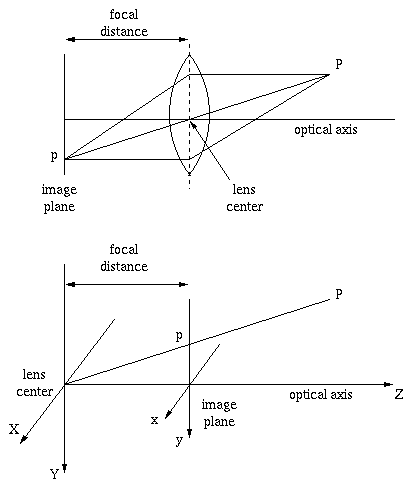
\includegraphics[scale=1]{images/pinhole}
\caption{Pinhole Camera Model}
\label{fig:jan}
\end{center}
\end{figure}


The transformation between world coordinates point P(X,Y,Z) and image coordinates p(x,y) is described as 
follows:

\begin{equation}
\label{eq:disparity2}
 x = \frac{f*X}{Z}
\end{equation}

\begin{equation}
\label{eq:disparity2}
 y = \frac{f*Y}{Z}
\end{equation}

This equations are  obtained using triangles similarity.

\section{Sensor Depth Calculation}

The Kinect sensor consists of an infrared laser emitter, an 
infrared camera and an RGB camera. The laser source emits a single 
beam which is split into multiple beams by a diffraction 
grating to create a constant 
pattern of speckles projected onto the scene. This pattern is 
captured by the infrared camera and is correlated against a 
reference pattern. The reference pattern is obtained by capturing 
a plane at a known distance from the sensor, and is stored in the 
memory of the sensor. When a speckle is projected on an object 
whose distance to the sensor is smaller or larger than that of the 
reference plane the position of the speckle in the infrared image 
will be shifted in the direction of the baseline between the laser 
projector and the perspective centre of the infrared camera. 
These shifts are measured for all speckles by a simple image 
correlation procedure, which yields a disparity image \cite{khoshelham2011accuracy} . For each 
pixel the distance to the sensor can then be retrieved from the 
corresponding disparity.



\begin{figure}[h!]
\begin{center}
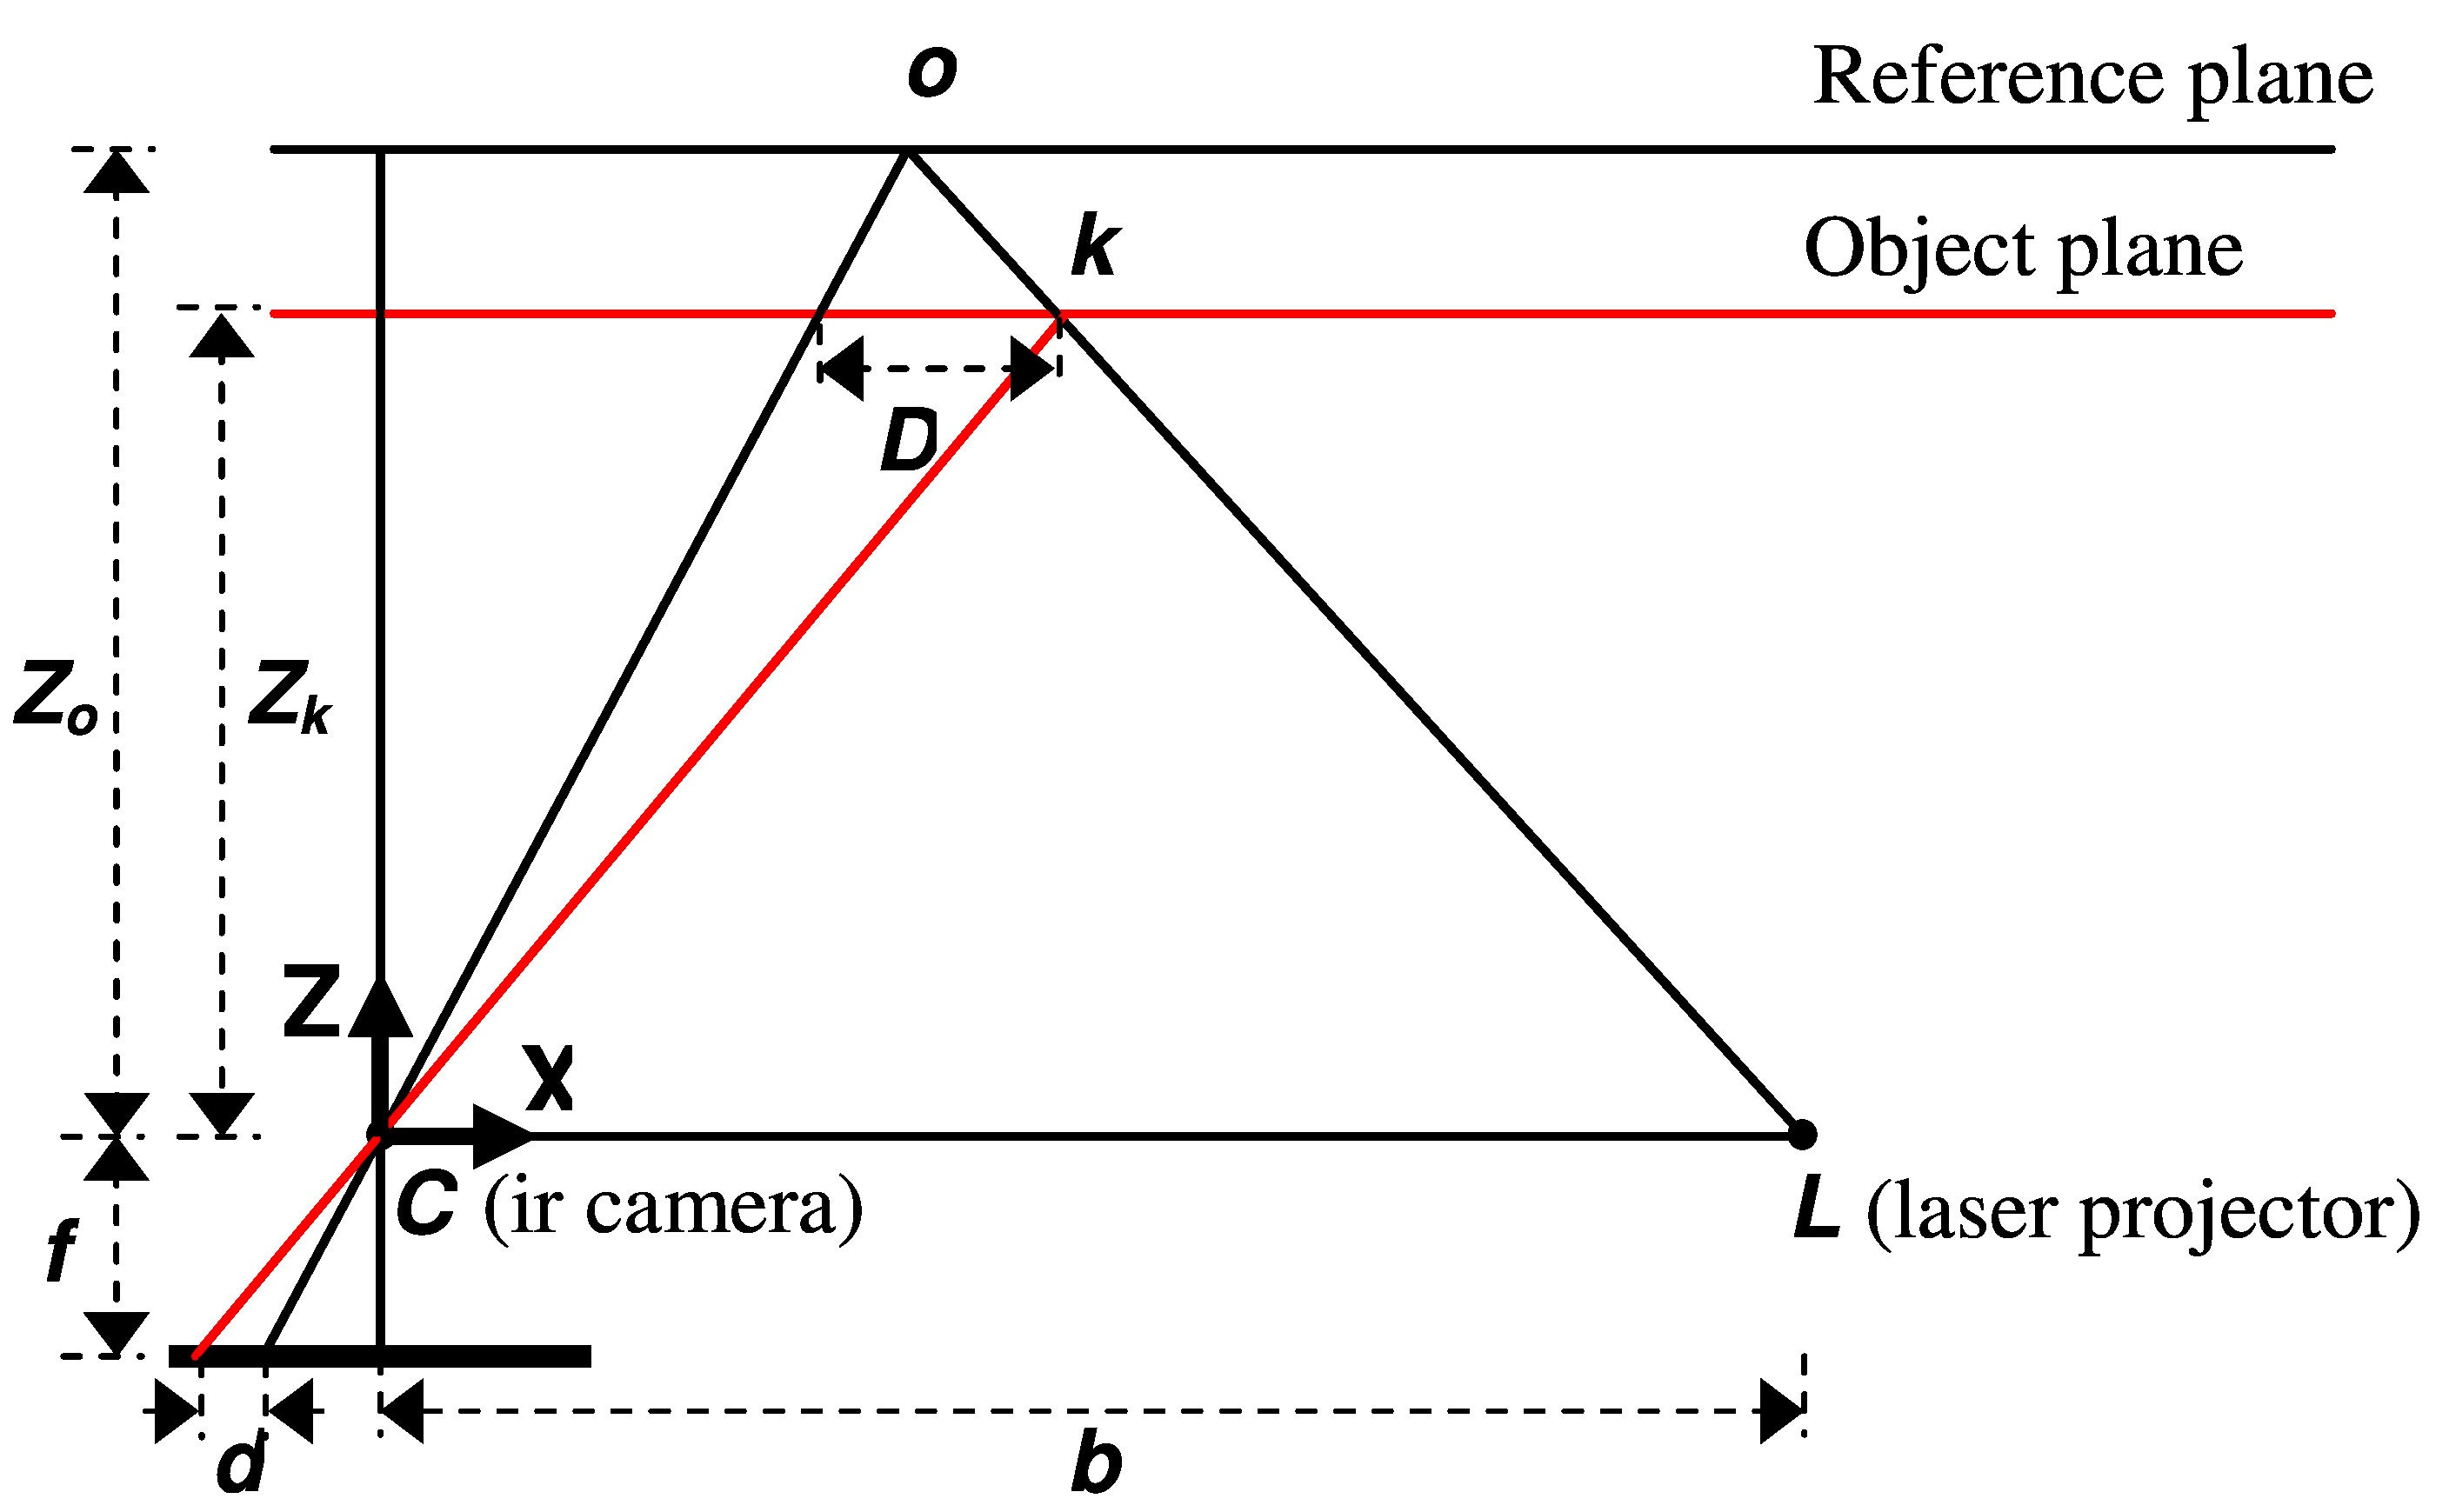
\includegraphics[scale=1]{images/kinect_triangulation}
\caption{Schematic representation of depth-disparity relation \cite{khoshelham2011accuracy}}
\label{fig:jan}
\end{center}
\end{figure}

\begin{equation}
\label{eq:disparity1}
 \frac{D}{b} = \frac{Z_0 - Z_k}{Z_0} 
\end{equation}


\begin{equation}
\label{eq:disparity2}
 \frac{d}{f} = \frac{D}{Z_k} 
\end{equation}


\section{Sensor Captured Data}

The sensor obtains two images: An RGB color image and a depth map.

The RGB color image has three channels: Red, Green and Blue. And each image color is generated 
combining this three colors. With a resolution of 640x480 pixels and 1 byte per channel. The sensor can 
capture color images at higher resolutions, but in our case we need just one color per depth map pixel.


The depth map is gray scale image and the intensity of each pixel is proportional to object distance. 
Most distant objects have greater intensitys than closer objects. The depth map is an image with a resolution of 
640x480 and one channel of 2 bytes.


The depth image data implicity contains the objects world coordinates, the relation between depth map 
and world coordinates is described as follows:

\begin{equation}
\label{eq:disparity2}
 X=\frac{(x-cx)*Z}{f}
\end{equation}

\begin{equation}
\label{eq:disparity2}
 Y=\frac{(y-cy)*Z}{f}
\end{equation}

\begin{equation}
\label{eq:disparity2}
 Z=\frac{depthVal}{factor}
\end{equation}

Where $(cx,cy)$ is the image principal point (projection of optical center on the image plane). f is the camera 
focal length, depthVal is the value of depth map at position $(x,y)$ of depth map image and factor is used to convert 
the depth value to real world distance in mm or m, depending on the software configuration. This factor is determined by 
the digital format used to store the depth data on the 
computer and it is dependant on the software used to access device data.
.


